\chapter{Codificação de Fonte}

A codificação de fonte sem perdas é o objetivo central quando
buscamos representar os símbolos de uma fonte estocástica de forma eficiente.
Ou seja, desejamos utilizar o menor número de bits possível para
codificar a informação produzida pela fonte, sem que haja perda de informação,
sendo assim possível reconstruir no receptor, exatamente a mesma mensagem
enviada pelo emissor.

O Teorema da Codificação de Shannon estabelece que, para uma fonte com entropia
$H(X)$, é possível codificar utilizando uma taxa $R > H(X)$ bits por símbolo,
desde que se empregue blocos suficientemente grandes. No entanto, a codificação
por blocos pode ser impraticável em aplicações reais devido à latência e à
complexidade computacional, o que motiva a busca por alternativas mais práticas
que ainda alcancem o limite teórico da entropia.

Neste capítulo, exploraremos duas abordagens principais: códigos de tamanho
variável, como a Codificação Huffman, que atribui palavras-código de
comprimento variável a símbolos individuais, e a codificação de fluxo
(\textit{stream coding}), que opera no fluxo de dados considerando o símbolo
atual e sua história, como na Codificação Aritmética e na Codificação
Lempel-Ziv --- esta última sendo universal, pois não requer conhecimento prévio
da distribuição $p(x)$. Assumiremos que a distribuição $p(x)$ da fonte é
conhecida ou que uma aproximação $q(x)$ está disponível, e investigaremos o
impacto de utilizar $q(x)$ quando a distribuição verdadeira é $p(x)$, sem
abordar diretamente o problema de estimação de $p(x)$. Buscaremos
analisar métodos práticos que se aproximem do limite de entropia.

Para abordar este assunto, devemos inicialmente fazer algumas definições.

Um código, no contexto de codificação de fonte, é uma função que mapeia os
símbolos de uma fonte em sequências de bits (palavras-código) de forma a
representá-los. Usualmente, o objetivo em se estabelecer um código é minimizar
o número de bits necessário para transmissão ou armazenamento da mensagem
produzida pela fonte. Um código pode ser de tamanho fixo ou variável, e, para
codificação sem perdas, devemos requerer que cada símbolo seja
univocamente recuperado a partir de sua palavra-código.

\begin{definition}[Codificação de Fonte]
Um código $C$ para a v.a. $X$ é um mapeamento de $\mathcal{X}$ em $\mathcal{D}^\ast$,
ou seja
\begin{equation}
  C: \mathcal{X} \rightarrow \mathcal{D}^\ast ,
\end{equation}
onde $\mathcal{D}^\ast$ é o conjunto
de sequências (\textit{strings}) finitas em um alfabeto $D$-ário. $C(x)$ é a palavra código
(\textit{codeword}) correspondente ao símbolo $x$, e $l(x)$ é o comprimento desta palavra.
\end{definition}
De forma geral, $\mathcal{D} = \{0,1, \ldots, D-1\}$, mas usualmente utilizamos $D=2$, ou seja,
codificação binária com alfabeto $\mathcal{D} = \{0,1\}$.
O conjunto $\mathcal{D}^\ast$ representa a extensão do alfabeto $\mathcal{D}$
(fecho de Kleene\footnote{
  O fecho de Kleene de um alfabeto $\mathcal{D}$, denotado $\mathcal{D}^\ast$,
  é um conceito da teoria de linguagens formais que inclui todas as sequências
  finitas que podem ser formadas concatenando zero ou mais símbolos de $\mathcal{D}$,
  incluindo a sequência vazia, frequentemente representada por $\epsilon$.

} do alfabeto), consistindo de todas as sequências finitas (de qualquer tamanho,
incluindo a sequência vazia) formadas por símbolos de $\mathcal{D}$, excluindo
sequências infinitas, que seriam denotadas por $\mathcal{D}^\infty$.

\begin{example}
Seja $\mathcal{X} = \{\text{azul}, \text{vermelho}\}$. O código pode ser $C(\text{vermelho})=00$ e
$C(\text{azul})=11$, o que seria um código binário para $\mathcal{D} = \{0,1\}$.
Teríamos então $\mathcal{D}^\ast = \{ 00 , 11 \}$. Uma sequência produzida pela fonte da forma
$(\text{azul},\text{azul},\text{vermelho})$ seria codificada como $(11,11,00)$, ou melhor, $111100$.
\end{example}

O comprimento esperado de um código é uma medida fundamental na codificação de
fonte, pois quantifica a eficiência média do código ao representar os símbolos
da fonte, permitindo comparar diferentes esquemas de codificação em termos de
uso de bits.

\begin{definition}[Comprimento Esperado]
O comprimento esperado $L(C)$ de um código $C$ para uma v.a. $X$ com distribuição $p(x)$ é dado por
\begin{equation}
  L(C) = \sum_x p(x) l(x) .
\end{equation}
\end{definition}


\begin{example}
  Seja $\mathcal{X} = \{1, 2, 3, 4\}$ e $\mathcal{D} = \{0, 1\}$. Podemos definir
  o código através da \Cref{tb:excode1}.
  \begin{table}[h]
    \centering
    \caption{Código binário de exemplo para quatro símbolos.}\label{tb:excode1}
    \begin{tabular}{c|c|c|c}
      x & p(x)  & c(x) & l(x) \\ \hline
      1 & $1/2$ & 0    & 1    \\
      2 & $1/4$ & 10   & 2    \\
      3 & $1/8$ & 110  & 3    \\
      4 & $1/8$ & 111  & 3    \\
    \end{tabular}
  \end{table}
  Neste caso, teremos $H(X) = 1.75$ e $L(C)=El(X)=1.75$, então este código é muito bom.
  A decodificação para este código é fácil, por exemplo, dada a sequência binária 010110111111110100,
  podemos prontamente identificar a sequência de símbolos que a produziu: 1,2,3,4,4,3,2,1.
  Seria como se tivéssemos uma pontuação separando os símbolos: 0,10,110,111,111,110,10,0.
  Dizemos que o código possui pontuação automática.
\end{example}

\begin{example}
Vamos considerar $\mathcal{X} = \{1,2,3\}$ e $\mathcal{D}=\{0,1\}$.
O código proposto é apresentado na \Cref{tb:excode2}.
\begin{table}[h]
  \centering
  \caption{Exemplo de código binário para um alfabeto com 3 símbolos.}\label{tb:excode2}
   \begin{tabular}{cccc}
   x      &  1    &   2   &   3   \\ \hline
   $p(x)$ & $1/3$ & $1/3$ & $1/3$ \\ \hline
   $C(X)$ & $0$   & $10$  & $11$
   \end{tabular}
\end{table}
Para o código proposto, teremos então $El(X)=1.66 > H$ bits, uma vez que $H = 1.58$ bits.
Note ainda como podemos facilmente decodificar uma sequência, como $10110010 = 2,3,1,1,2$.
\end{example}

A eficiência de um código é uma medida que compara o comprimento esperado $L$
do código com a entropia $H(X)$ da fonte. Ela serve como um indicativo do
quão próximo o código está do limite teórico de
compressão estabelecido pelo Teorema da Codificação de Shannon.

\begin{definition}[Eficiência de um código]
  A eficiência de um código é definida da seguinte forma
    \begin{equation}
      0 \leq \text{eficiência} \triangleq \frac{H_D(X)}{E l(X)} \leq 1 .
    \end{equation}
\end{definition}

\begin{example}
  Para $\mathcal{X} = \{1,2,3,4\}$ e $\mathcal{D}=\{0,1\}$ (código binário), considere os seguintes códigos
  dados na \Cref{tb:excode3}
  \begin{table}[h]
    \centering
    \caption{Comparativo de 4 códigos distintos para uma fonte com 4 símbolos e distribuição dada.}\label{tb:excode3}
    \begin{tabular}{c|c|c|c|c|c}
    $x$           & $p(x)$& $C_I$ & $C_{II}$ & $C_{III}$ & $C_{IV}$ \\ \hline
    1             & 0.5   &  0    &   0   &  0            &   0   \\
    2             & 0.25  &  0    &   1   & 10            &  01   \\
    3             & 0.125 &  1    &  00   & 110           & 011   \\
    4             & 0.125 & 10    &  11   & 111           & 0111  \\
    $H(X)$        & 1.75  &  -    &  -    &  -            &  -    \\
    $El(X)$       &  -    & 1.125 & 1.25  &  1.75         & 1.875 \\
    eficiência    &       & 1.555 & 1.4   & 1             & 0.933 
    \end{tabular}
  \end{table}
  Neste caso, obtemos valores impróprios para os códigos $C_I$ e $C_{II}$,
  indicando que não podem ser códigos sem perdas, já que violam do teorema de Shannon.
  O valor esperado do comprimento do código não pode ser menor que a entropia sem que o código incorra em erro.

  Note que o código $C_I$ não é unívoco. A sequência $00001$ pode ser decodificada como
  $1,2,1,2,3$ ou $2,1,2,1,3$ ou $1,1,1,1,3$.

  Considere $C_{II}$. O resultado da decodificação de $0011$ poderia ser $,1,1,2,2$ ou $3,4$ ou $3,2,2$ ou $1,1,4$.
  Novamente, não é possível decodificar sem que a probabilidade de erro seja nula (quando a sequência torna-se mais longa, a probabilidade de erro tende a $1$).

  O código $C_{III}$ é factível (já que $El \geq H$). O processo de decodificação é simples. Por exemplo: $111110100 = 111,110,10,0 = 4,3,2,1$.

  Utilizando o código $C_{IV}$ é possível decodificar a sequência $00000000111$ univocamente, porém os símbolos não são instantaneamente decodificados, é necessário analisar os bits à frente para conseguir decodificar.
\end{example}


\begin{definition}[Extensão de um código]
Um extensão $C^\ast$ de um código $C$ é um mapeamento de uma sequência finita
de símbolos em $\mathcal{X}$ em uma sequência finita de símbolos em $\mathcal{D}$ através da
concatenação dos códigos:
\begin{equation}
C^\ast (x_1,x_2,\ldots,x_n) = C(x_1) C(x_2) \ldots C(x_n) .
\end{equation}
\end{definition}

Um código não-singular é uma função de codificação que mapeia os símbolos de
uma fonte estocástica em palavras-código de forma que cada símbolo tenha uma
representação única, sendo essa uma condição necessária para a codificação sem
perdas, embora não garanta por si só a decodificação unívoca.

\begin{definition}[Código não-singular]
Um código é dito \textbf{não-singular} se todo elemento de $\mathcal{X}$
é mapeado em sequências (\textit{strings}) diferentes em $\mathcal{D}^\ast$. I.e.,
\begin{equation}
x_i \neq x_j \Rightarrow C(x_i) \neq C(x_j) .
\end{equation}
\end{definition}

Para garantir que cada sequência codificada possa ser recuperada de forma inequívoca
a partir de sua representação em bits, um código precisa ter decodificação unívoca,
ou seja, não pode haver ambiguidades na decodificação.

\begin{definition}[Código com decodificação unívoca]
Um código $C$ com extensão $C^\ast$ é decodificável univocamente se a sua extensão $C^\ast$ for não-singular.
\end{definition}

Em um código de prefixo nenhuma palavra-código é um prefixo de outra, garantindo que a decodificação possa ser realizada de
forma unívoca e sequencial sem a necessidade de olhar para além do próximo delimitador.

\begin{definition}[Código de prefixo]
Um código é chamado \emph{código de prefixo} ou \emph{código instantâneo} se nenhum palavra
é prefixo de qualquer outra palavra.
\end{definition}

Quando temos um código de prefixo, sabemos onde está o fim de uma palavra, pois ela não
é prefixo de nenhuma outra, ou seja, não existe nenhuma outra palavra que comece com a palavra
dada. Podemos dizer que um código de prefixo possui então a propriedade de auto-pontuação.

Dentre o conjunto dos códigos unívocos possíveis, queremos um código com
comprimento esperado mínimo possível. Analisando as classes de códigos,
intuitivamente pensamos que é mais provável encontrarmos um código com
comprimento esperado menor em uma classe maior (ou mais abrangente). 
A \Cref{fig:tiposcodigos} apresentado a estrutura hierárquica dos códigos
(todos os códigos $\supset$ não-singulares $\supset$ unicamente decodificáveis $\supset$ prefixo).

\begin{marginfigure}%
  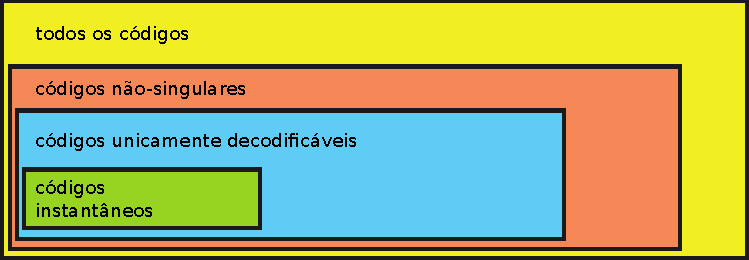
\includegraphics[width=\linewidth]{figures/tiposcodigos.pdf}
  \caption{Diagrama de representação dos conjuntos de códigos, evidenciando a estrutura hierárquica existente.}\label{fig:tiposcodigos}
\end{marginfigure}


A Desigualdade de Kraft estabelece uma condição necessária e suficiente para a
existência de códigos de prefixo com comprimentos de palavras-código
especificados. A demonstração, que será vista, ainda fornecerá um método para
construir um código de prefixo.

\begin{theorem}[Desigualdade de Kraft]
Para qualquer código instantâneo (código de prefixo) sobre um alfabeto de tamanho $D$, o comprimento
das palavras $l_1, l_2, \ldots, l_m$ deve satisfazer
      \begin{equation}
      \sum_i D^{-l_i} \leq 1 .
      \end{equation}
Por um outro lado, dado um conjunto de comprimentos de código satisfazendo a desigualdade acima,
então existe um código de prefixo com estes comprimentos.
\end{theorem}

Note que foi dito que existe um código de prefixo com aqueles comprimentos, não
significa que todos códigos cujos comprimentos satisfazem a desigualdade são
códigos de prefixo. Se existe um código não-instantâneo com comprimentos $l_i$
satisfazendo a desigualdade de Kraft, então podemos encontrar um outro código,
que terá a propriedade de prefixo, e que possuirá os mesmos comprimentos $l_i$,
consequentemente não alterando o comprimento esperado. Logo, será sempre melhor
escolher um código de prefixo.


\begin{proof}[Demonstração (Desigualdade de Kraft)]
Vamos representar o conjunto de códigos em uma árvore $D$-ária (não necessariamente balanceada),
conforme a \Cref{fig:Dtree}.

\begin{marginfigure}
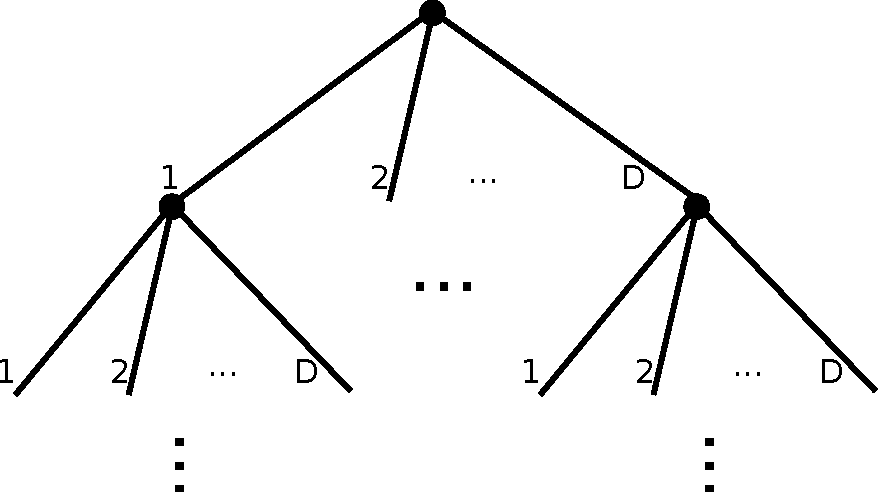
\includegraphics[width=\textwidth]{figures/Dtree.pdf}
\caption{Árvore $D$-ária.}\label{fig:Dtree}
\end{marginfigure}

As palavras correspondem à folhas na árvore. O caminho da raiz até a folha determina a palavra código.
A condição de prefixo implica que não existe uma palavra a não ser nas folhas
(nenhum descendente de uma palavra código será também uma palavra código).
$l_{\text{max}} = \max_i (l_i)$ é o comprimento da palavra mais longa.
Podemos expandir toda a árvore até o comprimento $l_{\text{max}}$.
Os nós no nível de $l_{\text{max}}$ são: palavras de código; descendentes de palavras de código; ou
apenas nós sem palavra código associada a ele ou seus antecessores.
Considere uma palavras $i$ no nível $l_i$ da árvore (então esta palavra possui comprimento $l_i$).
Existem então $D^{l_{\text{max}} - l_i}$ descendentes de $i$, na árvore, no nível $l_{\text{max}}$.
Com a condição de prefixo, podemos afirmar que os descendentes de código $i$ no nível $l_i$ são
disjuntos dos descendentes do código $j$ no nível $l_j$, quando $i \neq j$ (i.e., o conjunto de
descendentes para diferentes palavras é disjunto).
O número total de nós em um conjunto de todos descendentes é $\leq D^{l_{\text{max}}}$.
Utilizando o que vimos anteriormente, temos que a soma do número de descendentes de todos os códigos é menor ou
igual ao número de folhas na árvore cheia no nível $l_{\text{max}}$. Podemos então escrever
\begin{equation}
\sum_i D^{l_{\text{max}} - l_i} \leq D^{l_{\text{max}}} \quad \Rightarrow \quad \sum_i D^{-l_i} \leq 1 .
\end{equation}

Por outro lado, dados os comprimentos $l_1, l_2, \ldots, l_m$, satisfazendo Kraft, iremos mostrar como
construir um código de prefixo utilizando estes comprimentos.
Considere uma árvore $D$-ária cheia de profundidade $l_{\text{max}}$ e $D^{l_{\text{max}}}$ nós terminais.
Observe que: no nível 0 existe uma fração $1$ de descendentes de cada nó neste nível;
no nível 1 existe uma fração $1/D$ de descendentes de cada nó neste nível;
no nível 2 existe uma fração $1/D^2$ de descendentes de cada nó neste nível; e assim por diante.
De forma geral, em cada nível $i \in [0, l_{\text{max}}]$ da árvore, existe uma fração de $D^{-i}$
nós terminais que são descendentes de uma ramificação de cada um dos $D^i$ nós no nível $i$.
Ordene então os comprimentos $(l_1, l_2, \ldots, l_m)$ de forma ascendente $(s_1, s_2, \ldots, s_m)$,
sendo $s_1 \leq s_2 \leq \ldots \leq s_m$. Observe que existem tantos comprimentos quanto existem palavras.
Para o comprimento $s_1$, escolha um nó no nível $s_1$ para indicar o código.
Para garantir a condição de prefixo, o nó escolhido deve se tornar um nó terminal, eliminando assim uma
fração $D^{-s_1}$ de nós terminais no nível $l_{\text{max}}$.
Em seguida, escolha um dos nós remanescentes no nível $s_2$ (neste momento, existem $(D^{s_1}-1)D^{s_2-s_1}$
possíveis escolhas), eliminando assim uma fração $D^{-s_2}$ de nós terminais no nível $l_{\text{max}}$.
A fração total de nós eliminados, até o momento, foi de $D^{-s_1} + D^{-s_2}$.
Continuando este processo, iremos eliminar uma fração $\sum_{i=1}^{m} D^{-s_i}$ de nós, e neste processo
estamos garantindo que estamos criando um código instantâneo (uma palavra de código não pode ser prefixo de outra).
Como por suposição temos $\sum_{i=1}^{m} D^{-s_i} \leq 1$, nunca iremos eliminar mais do que todas as palavras
de código, então este processo não irá exaurir as palavras de código.
Criamos assim um código de prefixo com os comprimentos desejados, satisfazendo Kraft.
\end{proof}

